%%%%%%%%%%%%%%%%%%%%%%%%%%%%%%%%%%%%%%%%%
% Beamer Presentation
% LaTeX Template
% Version 1.0 (10/11/12)
%
% This template has been downloaded from:
% http://www.LaTeXTemplates.com
%
% License:
% CC BY-NC-SA 3.0 (http://creativecommons.org/licenses/by-nc-sa/3.0/)
%
%%%%%%%%%%%%%%%%%%%%%%%%%%%%%%%%%%%%%%%%%

%----------------------------------------------------------------------------------------
%	PACKAGES AND THEMES
%----------------------------------------------------------------------------------------

\documentclass{beamer}

\mode<presentation> {

% The Beamer class comes with a number of default slide themes
% which change the colors and layouts of slides. Below this is a list
% of all the themes, uncomment each in turn to see what they look like.

%\usetheme{default}
%\usetheme{AnnArbor}
%\usetheme{Antibes}
%\usetheme{Bergen}
%\usetheme{Berkeley}
%\usetheme{Berlin}
%\usetheme{Boadilla}
%\usetheme{CambridgeUS}
\usetheme{Copenhagen}
%\usetheme{Darmstadt}
%\usetheme{Dresden}
%\usetheme{Frankfurt}
%\usetheme{Goettingen}
%\usetheme{Hannover}
%\usetheme{Ilmenau}
%\usetheme{JuanLesPins}
%\usetheme{Luebeck}
%\usetheme{Madrid}
%\usetheme{Malmoe}
%\usetheme{Marburg}
%\usetheme{Montpellier}
%\usetheme{PaloAlto}
%\usetheme{Pittsburgh}
%\usetheme{Rochester}
%\usetheme{Singapore}
%\usetheme{Szeged}
%\usetheme{Warsaw}

% As well as themes, the Beamer class has a number of color themes
% for any slide theme. Uncomment each of these in turn to see how it
% changes the colors of your current slide theme.

%\usecolortheme{albatross}
%\usecolortheme{beaver}
%\usecolortheme{beetle}
%\usecolortheme{crane}
%\usecolortheme{dolphin}
%\usecolortheme{dove}
%\usecolortheme{fly}
%\usecolortheme{lily}
%\usecolortheme{orchid}
%\usecolortheme{rose}
%\usecolortheme{seagull}
%\usecolortheme{seahorse}
%\usecolortheme{whale}
%\usecolortheme{wolverine}

%\setbeamertemplate{footline} % To remove the footer line in all slides uncomment this line
\setbeamertemplate{footline}[page number] % To replace the footer line in all slides with a simple slide count uncomment this line

\setbeamertemplate{navigation symbols}{} % To remove the navigation symbols from the bottom of all slides uncomment this line
}

\usepackage{graphicx} % Allows including images
\usepackage{booktabs} % Allows the use of \toprule, \midrule and \bottomrule in tables
\usepackage[utf8]{inputenc}
\usepackage[labelformat=empty]{caption}
\usepackage{subcaption}
\usepackage{multicol}

%----------------------------------------------------------------------------------------
%	TITLE PAGE
%----------------------------------------------------------------------------------------

\title[Seleção de Comportamento]{Aprendizagem por Reforço aplicada a Seleção de Comportamento em Robótica Móvel} % The short title appears at the bottom of every slide, the full title is only on the title page

\author{Tiago Pimentel Martins da Silva} % Your name
\institute[UnB] % Your institution as it will appear on the bottom of every slide, may be shorthand to save space
{
Universidade de Brasília \\ % Your institution for the title page
\medskip
\textit{tiagopms@gmail.com} % Your email address
}
\date{December 8, 2014} % Date, can be changed to a custom date

\AtBeginSubsection[]{
  \frame<beamer>{ 
    %\frametitle{Overview}   
    \tableofcontents[currentsection,currentsubsection] 
  }
}

\begin{document}

\begin{frame}
\titlepage % Print the title page as the first slide
\end{frame}

\begin{frame}
%\frametitle{Overview} % Table of contents slide, comment this block out to remove it
\tableofcontents % Throughout your presentation, if you choose to use \section{} and \subsection{} commands, these will automatically be printed on this slide as an overview of your presentation
\end{frame}

%----------------------------------------------------------------------------------------
%	PRESENTATION SLIDES
%----------------------------------------------------------------------------------------

%------------------------------------------------
\section{Motivação} % Sections can be created in order to organize your presentation into discrete blocks, all sections and subsections are automatically printed in the table of contents as an overview of the talk
%------------------------------------------------

\subsection{Contextualização} % A subsection can be created just before a set of slides with a common theme to further break down your presentation into chunks

\begin{frame}
%\frametitle{Introdução}
A automação pode ser resumida por uma pergunta:
\pause
\textit{O que devo fazer a seguir, sabendo o que já vi e o que fiz?}
\pause
\\~\\

Nesse trabalho, tentaremos responder essa pergunta utilizando:\pause

\begin{itemize}
	\item Planejamento de tarefas;\pause
	\item Redes bayesianas;\pause
	\item Aprendizagem por reforço.
\end{itemize}
\end{frame}

%------------------------------------------------

\subsection{Trabalhos anteriores}

\begin{frame}
%\frametitle{Koike}
Koike (2008) \cite{Koike:2008}
\begin{itemize}
	\item Seleção de comportamentos;
	\item Redes bayesianas.
\end{itemize}\pause

Lidoris (2011) \cite{lidoris2011state}
\begin{itemize}
	\item Seleção de comportamentos;
	\item Redes bayesianas;
	\item Aprendizagem por demonstração.
\end{itemize}
\end{frame}

%------------------------------------------------
\section{Fundamentação Teórica}
%------------------------------------------------

\subsection{Filtro Bayesiano}

\begin{frame}
%\frametitle{Lidoris}
\begin{overprint}
\onslide<+|handout:0>
\begin{itemize}
	\item Estimar a distribuição conjunta de probabilidade:
\end{itemize}

$$ P \left( M^{0:t} S^{0:t} Z^{0:t} | \pi_f \right) $$
\onslide<+|handout:0>
\begin{itemize}
	\item Estimar a distribuição conjunta de probabilidade;
	\item Pode ser descrita por:
\end{itemize}

$$
	P ( M^{0: t} S^{0: t} Z^{0: t} \mid \pi_f ) = P ( M^0 S^0 Z^0 \mid \pi_f ) \cdot \prod\limits_{j =1}^{t} 
        \left(
            \begin{array}{l}
                P( S^j \mid S^{j -1} M^{j -1} \pi_f ) \\
                \times P( Z^j \mid S^j \pi_f ) \\
                \times P( M^j \mid S^j M^{j -1} \pi_f )
            \end{array}
        \right)
$$
\end{overprint}

\end{frame}

%------------------------------------------------

\begin{frame}
%\frametitle{Lidoris}
Dividido em três passos:
\begin{itemize}
	\item Predição: $$
	\textcolor{green}{ P \left( S^t \mid z^{0: t-1} m^{0: t-1} \pi_f \right) } \propto \sum\limits_{S^{t-1}}
        \left(
            \begin{array}{l}
                P \left( S^t \mid S^{t-1} m^{t-1} \pi_f \right) \\
                \times P \left( m^{t-1} \mid S^{t-1} m^{t-2} \pi_f \right)\\
                \times \textcolor{blue}{ P \left( S^{t-1} \mid z^{0: t-1} m^{0: t-2} \pi_f \right) }
            \end{array}
        \right)
    $$\pause
	\item Observação: $$
	\textcolor{blue}{ P \left( S^t \mid z^{0: t} m^{0: t-1} \pi_f \right) } \propto 
        \left(
            \begin{array}{l}
                P \left( z^t \mid S^t \pi_f \right) \\
                \times \textcolor{green}{ P \left( S^t \mid z^{0: t-1} m^{0: t-1} \pi_f \right) }
            \end{array}
        \right)
    $$\pause
	\item Escolha de ação motora: $$
	\textcolor{brown}{ P \left( M^t \mid z^{0: t} m^{0: t-1} \pi_f \right) } \propto \sum\limits_{S^t}
        \left(
            \begin{array}{l}
                P \left( M^t \mid S^t m^{t-1} \pi_f \right)\\
                \times \textcolor{blue}{ P \left( S^t \mid z^{0: t} m^{0: t-1} \pi_f \right) }
            \end{array}
        \right)
    $$
\end{itemize}
\end{frame}

%------------------------------------------------

\begin{frame}
%\frametitle{Lidoris}

\begin{figure}[h]
    \centering
    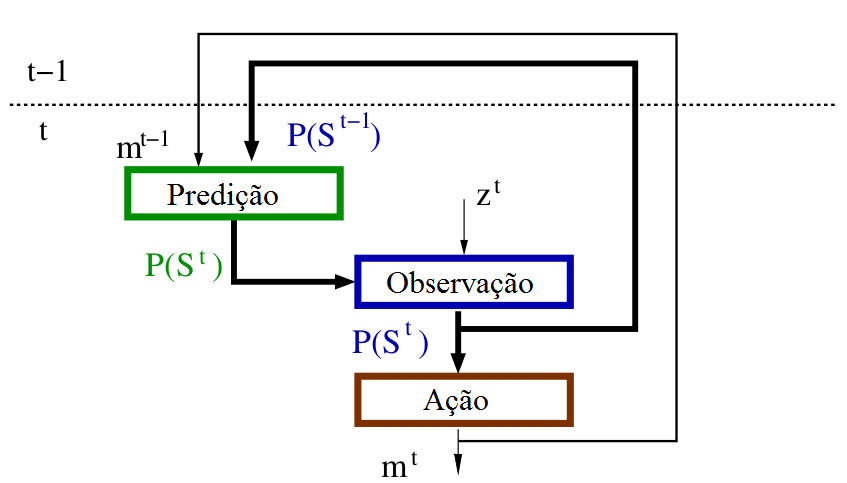
\includegraphics[width=\linewidth]{images/modelo_bayesiano-carla}
    \caption{\label{img:ModeloProbabilisticoCarla}Filtro Bayesiano Recursivo. Fonte: \cite{Koike:2005}}
\end{figure}
\end{frame}

%------------------------------------------------

\subsection{MDP (Processo de Decisão de Markov)}

\begin{frame}
%\frametitle{Lidoris}

\begin{itemize}
	\item Base matemática para o modelamento de tomada de decisões;\pause
	\item Extensão de cadeias de Markov;\pause
	\item Possui ações e recompensas (escolha e motivação);\pause
	\item Cálculo recursivo.
\end{itemize}
\end{frame}

%------------------------------------------------

\begin{frame}
%\frametitle{Lidoris}
Necessário:
\begin{itemize}
	\item Modelo de atuação: $$ P \left(s' | u, s \right) $$\pause
	\item Modelo de recompensas: $$ r \left( s, u, s' \right) $$
\end{itemize}
\end{frame}

%------------------------------------------------

\begin{frame}
%\frametitle{Lidoris}

\begin{itemize}
	\item Inicialmente, calcula-se um valor de ganho (analisando apenas a próxima ação): $$ V_1 \left( s \right) = \underset{u}{max} \left( \int \! r \left( s, u, s' \right) \cdot P \left( s' \mid u, s \right) \, \mathrm{d}s' \right) $$\pause
	\item E escolhe-se uma ação que maxime esse ganho: $$ \pi_1 \left( s \right) = \underset{u}{argmax} \left( \int \! r \left( s, u, s' \right) \cdot P \left( s' \mid u, s \right) \, \mathrm{d}s' \right) $$
\end{itemize}
\end{frame}

%------------------------------------------------

\begin{frame}
%\frametitle{Lidoris}

\begin{itemize}
	\item Depois, calcula-se esse valor de ganho iterativamente (analisando mais ações futuras): $$ V_j \left( s \right) = \underset{u}{max} \left( \int \! \left( r \left( s, u, s' \right) + \gamma \cdot V_{j-1} \left( s' \right) \right) \cdot P \left( s' \mid u, s \right) \, \mathrm{d}s' \right) $$\pause
	\item E escolhe-se uma ação que maxime esse ganho: $$ \pi_j \left( s \right) = \underset{u}{argmax} \left( \int \! \left( r \left( s, u, s' \right) + \gamma \cdot V_{j-1} \left( s' \right) \right) \cdot P \left( s' \mid u, s \right) \, \mathrm{d}s' \right) $$\pause
	\item Para $ j \rightarrow \infty $ a política $ \pi_j \left( s \right) $ tende a ser ótima.
\end{itemize}
\end{frame}


%------------------------------------------------

\subsection{TD (Diferença Temporal)}

\begin{frame}
%\frametitle{Lidoris}
\begin{itemize}
	\item Estima o valor de $ V \left( s \right) $;\pause
	\item Não se tem o modelo de atuação $ P \left(s' | u, s \right) $
	ou de recompensa $ r \left( s, u, s' \right) $;\pause
	\item Aprende-se os valores a partir de experiências reais;\pause
	\item É necessário ter uma política $ \pi_{td} \left( s \right) $ pré definida e fixa.
\end{itemize}
\end{frame}

%------------------------------------------------

\begin{frame}
%\frametitle{Lidoris}
Inicialmente:
$$V_{\pi_{td}}^0 \left( s \right) = 0 , \forall s \in S $$\pause
Para cada experiência $ \left( s, u, s', r \right) $:\pause
\begin{itemize}
	\item Obtém-se um valor $ amostra $:
		$$ amostra = r + \gamma \cdot V_{\pi_{td}}^{t-1} \left( s' \right) $$\pause
	\item Atualiza-se o valor de ganho para o estado $ s $:
		$$ V_{\pi_{td}}^t \left( s \right) = \left( 1 - \alpha \right) \cdot V_{\pi_{td}}^{t-1} \left( s \right) + \alpha \cdot amostra $$\pause
	\item Para $ t \rightarrow \infty $, $ V_{\pi_{td}}^t \left( s \right) $ tende ao valor obtido no MDP, para uma política $ \pi_{td} $ ótima.
\end{itemize}
\end{frame}

%------------------------------------------------

\subsection{Q Learning}

\begin{frame}
%\frametitle{Lidoris}
\begin{itemize}
	\item Estima o valor de $ Q \left( s, u \right) $, sendo $ Q $ o valor de ganho para cada par estado-ação:
		$$ V \left( s \right) = \underset{u}{max} \left( Q \left( s, u \right) \right) $$\pause
	\item Não se tem o modelo de atuação $ P \left(s' | u, s \right) $
	ou de recompensa $ r \left( s, u, s' \right) $;\pause
	\item Aprende-se os valores a partir de experiências reais;\pause
	\item Aprende-se uma política $ \pi \left( s \right) $ ótima.
\end{itemize}
\end{frame}

%------------------------------------------------

\begin{frame}
%\frametitle{Lidoris}
Inicialmente:
$$ Q^0 \left( s, u \right) = 0 , \forall \left( s, u \right) \in \left( S, U \right) $$\pause
Para cada experiência $ \left( s, u, s', r \right) $:\pause
\begin{itemize}
	\item Obtém-se um valor $ amostra $:
		$$ amostra = r + \gamma \cdot \underset{u}{max} \left( Q^{t-1} \left( s', u' \right) \right) $$\pause
	\item Atualiza-se o valor de ganho para o par estado-ação $ \left( s, u \right) $:
		$$ Q^t \left( s, u \right) = \left( 1 - \alpha \right) \cdot Q^{t-1} \left( s, u \right) + \alpha \cdot amostra $$\pause
	\item Para $ t \rightarrow \infty $, uma política $ \pi \left( s \right) $ é ótima se obtida com a função:
		$$ \pi^t \left( s \right) = \underset{u}{argmax} \left( Q^t \left( s, u \right) \right) $$
\end{itemize}
\end{frame}

%------------------------------------------------

\begin{frame}
%\frametitle{Lidoris}
Limitações:\pause
\begin{itemize}
	\item Podem existir muitos estados para se visitar: em um espaço contínuo, por exemplo, seriam infinitos;\pause
	\item Podem existir muitas ações possíveis para cada estado: para o acionamento analógico de um motor, por exemplo, seriam infinitas;\pause
	\item Se houverem muitos pares ação-estado $ \left( S, U \right) $, mesmo que seja possível aprender por um tempo muito grande, é necessário armazenar o valor de $ Q \left( S, U \right) $ para cada um desses pares;\pause
	\item O algoritmo não consegue aplicar o que aprendeu em um estado para outros estados com características similares.
\end{itemize}
\end{frame}

%------------------------------------------------

\begin{frame}
%\frametitle{Lidoris}
Pode-se generalizar os pares estado-ação utilizando-se características deles:
$$ Q \left( S, U \right) = \omega_1 \cdot f_1 \left( S, U \right) + \omega_2 \cdot f_2 \left( S, U \right) + \cdots + \omega_n \cdot f_n \left( S, U \right) $$\pause
Para cada experiência $ \left( s, u, s', r \right) $:\pause
\begin{itemize}
	\item Obtém-se um valor $ erro $:
		$$ erro = r + \gamma \cdot \underset{u}{max} \left( Q^{t-1} \left( s', u' \right) \right) - Q^{t-1} \left( s, u \right) $$\pause
	\item Atualiza-se o valor de ganho para o par estado-ação $ \left( s, u \right) $:
		$$ \omega_i^t = \omega_i^{t-1} + \alpha \cdot erro \cdot f_i \left( s, u \right) $$
\end{itemize}
\end{frame}

%------------------------------------------------
\section{Solução Implementada}
%------------------------------------------------

\subsection{Seleção de comportamentos}

\begin{frame}
%\frametitle{Lidoris}
Análogamente à aprendizagem com os pares estado-ação $ \left( S, U \right) $, pode-se utilizar pares estado-comportamento $ \left( S, B \right) $:
$$ Q \left( S, B \right) = \omega_1 \cdot f_1 \left( S, B \right) + \omega_2 \cdot f_2 \left( S, B \right) + \cdots + \omega_n \cdot f_n \left( S, B \right) $$\pause
Agora, para cada experiência $ \left( s, b, s', r \right) $:\pause
\begin{itemize}
	\item Obtém-se um valor $ erro $:
		$$ erro = r + \gamma \cdot \underset{b}{max} \left( Q^{t-1} \left( s', b' \right) \right) - Q^{t-1} \left( s, b \right) $$\pause
	\item Atualiza-se todos os pesos $ \omega_i $ de acordo com o valor de suas características $ f_i \left( s, b \right) $:
		$$ \omega_i^t = \omega_i^{t-1} + \alpha \cdot erro \cdot f_i \left( s, b \right) $$
\end{itemize}
\end{frame}

%------------------------------------------------

\subsection{Sistema Parcialmente Observável}

\begin{frame}
\begin{itemize}
	\item \textit{Q Learning} foi criado para um sistema completamente observável;\pause
	\item Não sabemos o estado atual;\pause
	\item Essa definição então é expandida pra um sistema parcialmente observável;\pause
	\item Utiliza-se $ a \in A $ no lugar de $ s \in S $;\pause
	\item $ a \in A $ é uma distribuição de probabilidades de se encontrar nos estados $ s \in S $.
\end{itemize}
\end{frame}

%------------------------------------------------

\begin{frame}
%\frametitle{Lidoris}
Análogamente à aprendizagem anterior, com os pares estado-ação $ \left( S, U \right) $, pode-se utilizar pares (distribuição de probabilidade para os estados, comportamento) $ \left( A, B \right) $:
$$ Q \left( A, B \right) = \omega_1 \cdot f_1 \left( A, B \right) + \omega_2 \cdot f_2 \left( A, B \right) + \cdots + \omega_n \cdot f_n \left( A, B \right) $$\pause
Agora, para cada experiência $ \left( a, b, a', r \right) $:\pause
\begin{itemize}
	\item Obtém-se um valor $ erro $:
		$$ erro = r + \gamma \cdot \underset{b}{max} \left( Q^{t-1} \left( a', b' \right) \right) - Q^{t-1} \left( a, b \right) $$\pause
	\item Atualiza-se todos os pesos $ \omega_i $ de acordo com o valor de suas características $ f_i \left( a, b \right) $:
		$$ \omega_i^t = \omega_i^{t-1} + \alpha \cdot erro \cdot f_i \left( a, b \right) $$
\end{itemize}
\end{frame}

%------------------------------------------------

\subsection{Abordagem Bayesiana Final}

\begin{frame}
Para incorporar a seleção de comportamento no filtro bayesiano, expande-se as definições de:\pause
\begin{itemize}
	\item Observação: $$ Z^+ = \binom{Z}{Z_b} = \binom{Z}{B} $$\pause
	\item Estado: $$ S^+ = \binom{S}{S_b} $$
\end{itemize}
\end{frame}

%------------------------------------------------

\begin{frame}
O sistema final possui duas partes, cada uma dividida em passos:\pause
\begin{itemize}
	\item Treinamento
	\begin{itemize}
		\item Predição;
		\item Observação;
		\item Seleção de comportamento;
		\item Seleção de ação motora;
		\item Aprendizagem.\pause
	\end{itemize}
	\item Pós treinamento
	\begin{itemize}
		\item Predição;
		\item Observação;
		\item Seleção de comportamento;
		\item Seleção de ação motora
	\end{itemize}
\end{itemize}
\end{frame}

%------------------------------------------------

\begin{frame}
Predição:
$$
    \resizebox{.9\hsize}{!}{ $
    		\textcolor{green}{ P \left( S^t S_b^t \mid z^{0: t-1} b^{0: t-1} m^{0: t-1} \pi_f \right) } \propto \sum\limits_{S^{t-1} S_b^{t-1}}
        \left(
            \begin{array}{l}
                P \left( S^t \mid S^{t-1} m^{t-1} \pi_f \right) \times P \left( S_b^t \mid \pi_f \right) \\
                \times P \left( m^{t-1} \mid S^{t-1} S_b^{t-1} m^{t-2} \pi_f \right)\\
                \times \textcolor{blue}{ P \left( S^{t-1} S_b^{t-1} \mid z^{0: t-1} b^{0: t-1} m^{0: t-2} \pi_f \right) }
            \end{array}
        \right) $}
$$\pause
Seleção de Comportamento:
$$
    \resizebox{.8\hsize}{!}{ $
    		\textcolor{red}{ Q^t \left( a^t, B^t \right) } = \textcolor{violet}{ \omega_1 } \cdot f_1 \left( a^t, B^t \right) + \textcolor{violet}{ \omega_2 } \cdot f_2 \left( a^t, B^t \right) + \cdots + \textcolor{violet}{ \omega_n } \cdot f_n \left( a^t, B^t \right)
    $}
$$\pause
Observação:
$$
    \resizebox{.8\hsize}{!}{ $
    		\textcolor{blue}{ P \left( S^t S_b^t \mid z^{0: t} b^{0: t} m^{0: t-1} \pi_f \right) } \propto
        \left(
            \begin{array}{l}
                P \left( z^t \mid S^t \pi_f \right) \times P \left( b^t \mid S_b^t \pi_f \right) \\
                \times \textcolor{green}{ P \left( S^t S_b^t \mid z^{0: t-1} b^{0: t-1} m^{0: t-1} \pi_f \right) }
            \end{array}
        \right)
    $}
$$\pause
Seleção de ação motora:
$$
    \resizebox{.8\hsize}{!}{ $
    		\textcolor{brown}{ P \left( M^t \mid z^{0: t} b^{0: t} m^{0: t-1} \pi_f \right) } \propto \sum\limits_{S^t S_b^t}
        \left(
            \begin{array}{l}
                P \left( M^t \mid S^t S_b^t m^{t-1} \pi_f \right)\\
                \times \textcolor{blue}{ P \left( S^t S_b^t \mid z^{0: t} b^{0: t} m^{0: t-1} \pi_f \right) }
            \end{array}
        \right)
    $}
$$\pause
Aprendizagem:
$$
    \resizebox{.7\hsize}{!}{ $
    		erro = r + \gamma \cdot \underset{b'}{max} \left( Q^{t-1} \left( a^t, b' \right) \right) - \textcolor{red}{ Q^{t-1} \left( a^{t-1}, b^{t-1} \right) }
    $}
$$
$$
    \resizebox{.5\hsize}{!}{ $
    		\textcolor{violet}{ \omega_i^t } = \omega_i^{t-1} + \alpha \cdot erro \cdot f_i \left( a^{t-1}, b^{t-1} \right)
    $}
$$
\end{frame}

%------------------------------------------------

\begin{frame}
Treinamento:

\begin{figure}[H]
    \centering
    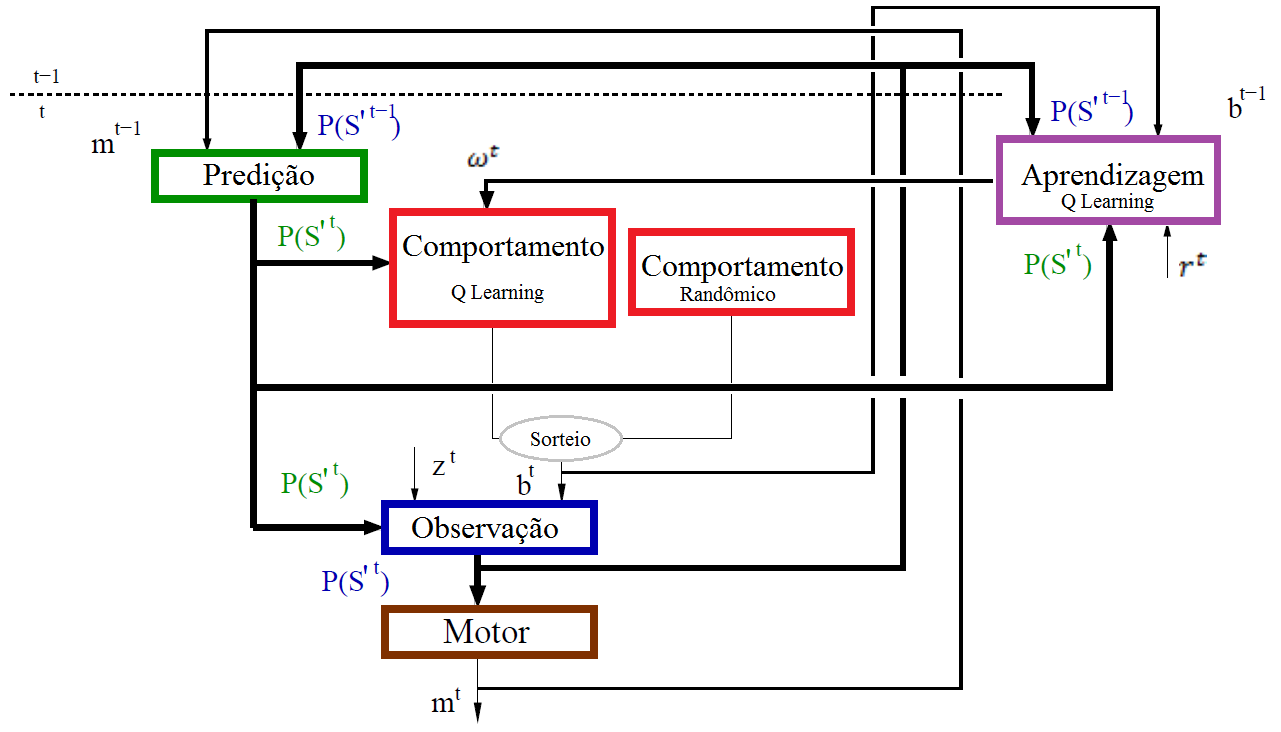
\includegraphics[width=\linewidth]{images/modelo_bayesiano_treino-tiago}
    \caption{Filtro Bayesiano utilizando \textit{Q Learning} para Seleção de Comportamento. Durante treinamento.}
    \label{img:ModeloFinalTreinamento}
\end{figure}
\end{frame}

%------------------------------------------------

\begin{frame}
Pós treinamento:

\begin{figure}[h!]
    \centering
    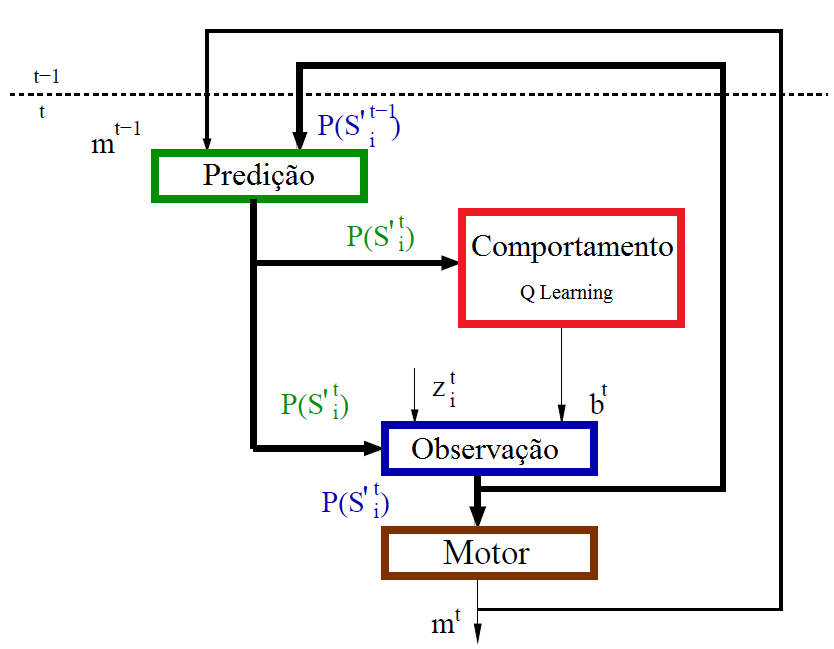
\includegraphics[height=0.7\textheight]{images/modelo_bayesiano_final-tiago}
    \caption{Filtro Bayesiano utilizando \textit{Q Learning} para Seleção de Comportamento. Após treinamento completo.}
    \label{img:ModeloFinalPosTreinamento}
\end{figure}
\end{frame}

%------------------------------------------------

\subsection{Plataforma de testes}

\begin{frame}
\begin{itemize}
	\item Plataforma de Pacman%
		\footnote{Essa plataforma foi desenvolvida em Berkeley para aulas de IA e pode ser encontrada em http://ai.berkeley.edu/project\_overview.html%
		} em Python;
	\item Código desevolvido em C++;
	\item Integração feita utilizando ROS.
\end{itemize}

\begin{figure}[h]
    \centering
    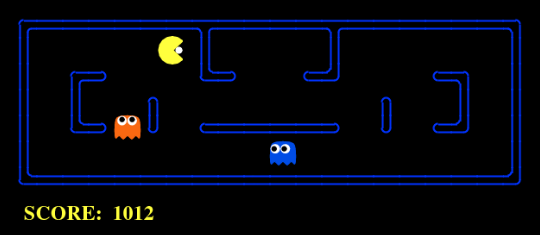
\includegraphics[width=0.7\linewidth]{images/pacman_platform}
    \caption{\label{img:PlataformaSimulacaoPacman}Plataforma do jogo Pacman.}
\end{figure}
\end{frame}

%------------------------------------------------

\begin{frame}
Quatro mensagens trocadas:\pause
\begin{itemize}
	\item Posição do agente (Pacman) --- $ \left( x, y \right) \in \mathbb{R}^2 $;\pause
	\item Distância para os fantasmas --- $ \left( d_x, d_y \right) = \left( \Delta x, \Delta y \right) \in \mathbb{R}^2 $;\pause
	\item Ação a ser executada --- $ m \in \left\{Norte, Sul, Leste, Oeste, Esperar \right\} $;\pause
	\item Recompensa recebida do ambiente --- $ r \in \mathbb{R} $.
\end{itemize}
\end{frame}

%------------------------------------------------

\begin{frame}
Erros inseridos:\pause
\begin{itemize}
	\item Posição do agente (Pacman) --- Erro gaussiano;\pause
	\item Distância para os fantasmas --- Erro gaussiano;\pause
	\item Ação a ser executada --- Chance $ \nu_{atuacao} $ de ação desejada ser executada (se não, é executada ação aleatória);\pause
	\item Recompensa recebida do ambiente --- Nenhum erro inserido.
\end{itemize}
\end{frame}

%------------------------------------------------
\section{Resultados}
%------------------------------------------------

\subsection{3 Comportamentos no mapa pequeno (Teste 1)}

\begin{frame}
\begin{multicols}{2}
Comportamentos:
\begin{itemize}
	\item Ficar Parado;
	\item Comer;
	\item Fugir.
\end{itemize}

Características ($ f_i \left( a, B \right) $):
\begin{itemize}
	\item Bias;
	\item Distância para Comida;
	\item Probabilidade de Fantasma.
\end{itemize}

\end{multicols}

\begin{figure}[h]
    \centering
    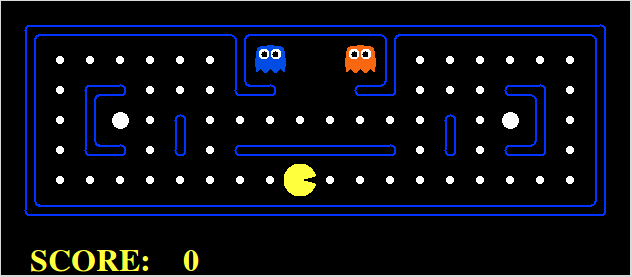
\includegraphics[width=0.6\linewidth]{images/pacman_small_map}
    \caption{Mapa pequeno do jogo Pacman.}
    \label{img:PlataformaPacmanMapaPequeno}
\end{figure}
\end{frame}

%------------------------------------------------

\begin{frame}
$$
    \resizebox{.8\hsize}{!}{ $
    		\textcolor{red}{ Q^t \left( a^t, B^t \right) } = \textcolor{violet}{ \omega_1 } \cdot f_1 \left( a^t, B^t \right) + \textcolor{violet}{ \omega_2 } \cdot f_2 \left( a^t, B^t \right) + \textcolor{violet}{ \omega_3 } \cdot f_3 \left( a^t, B^t \right)
    $}
$$\pause
\begin{figure}[h]
	\centering
	\begin{subfigure}[t]{.5\textwidth}
		\centering
		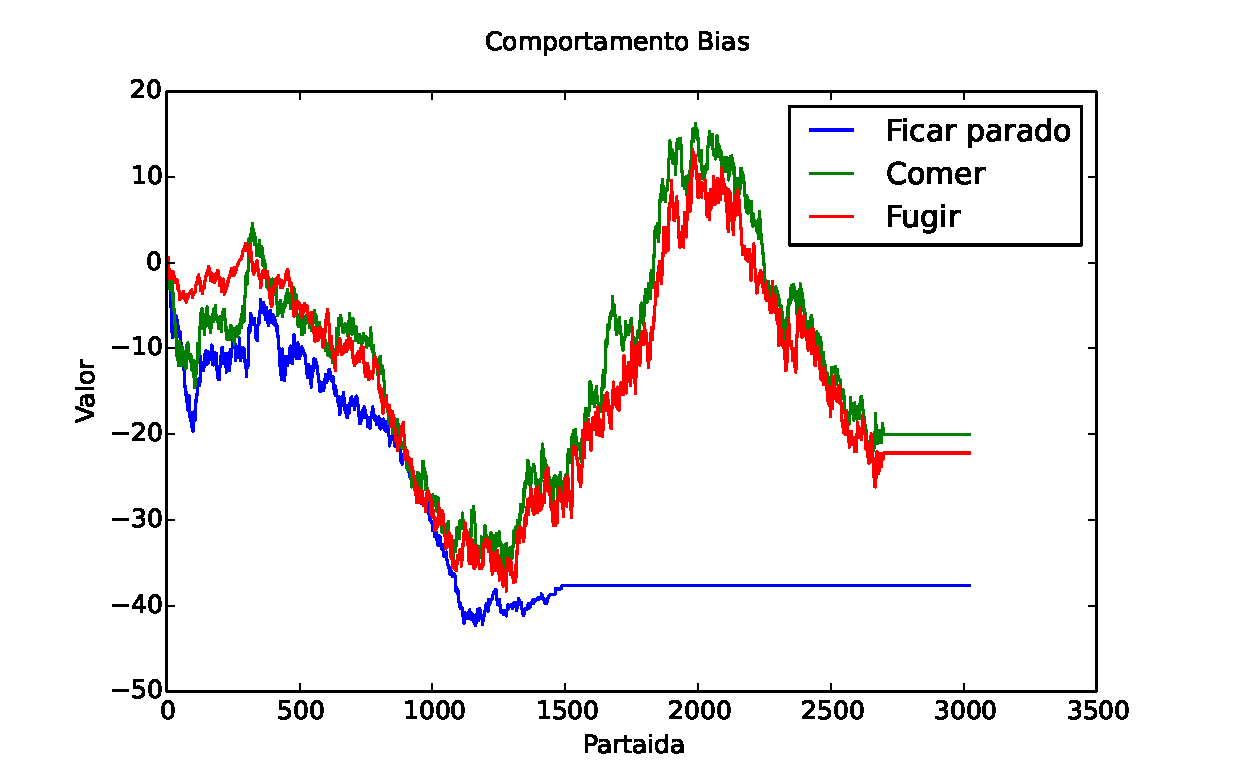
\includegraphics[width=.6\linewidth]{images/3_behaviors_small_map/weights____pol__Bias}
		\caption{Bias ($ \omega_1 $)}
		\label{img:3ComportamentosMapaPequeno:PesoBias}
	\end{subfigure}%
	\begin{subfigure}[t]{.5\textwidth}
		\centering
		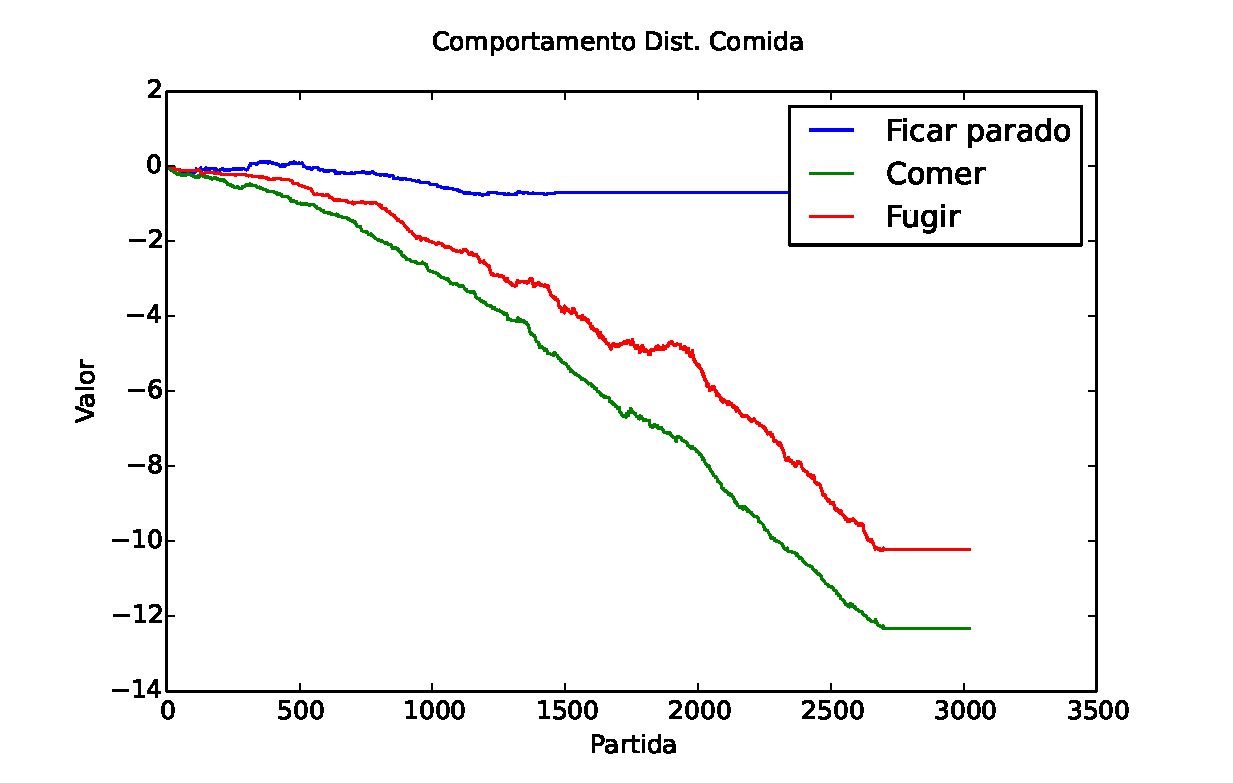
\includegraphics[width=.6\linewidth]{images/3_behaviors_small_map/weights____pol__DistComida}
		\caption{Distância para Comida ($ \omega_2 $)}
		\label{img:3ComportamentosMapaPequeno:PesoDistComida}
	\end{subfigure}
	\begin{subfigure}[t]{\textwidth}
		\centering
		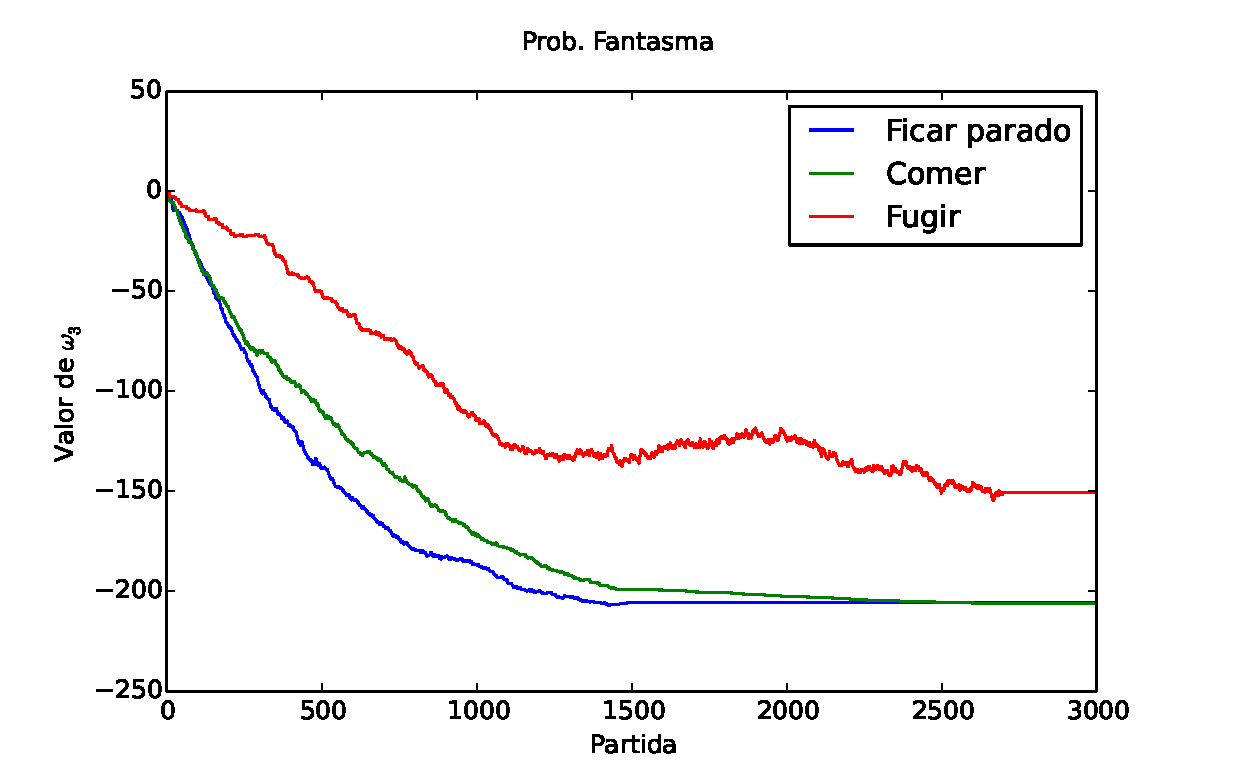
\includegraphics[width=.3\linewidth]{images/3_behaviors_small_map/weights____pol__ProbFantasma}
		\caption{Probabilidade de Fantasma} ($ \omega_3 $)
	\end{subfigure}
	\label{img:3ComportamentosMapaPequeno:PesoBiasAndDistComida}
\end{figure}
\end{frame}

%------------------------------------------------

\begin{frame}
\begin{figure}[h]
    \centering
    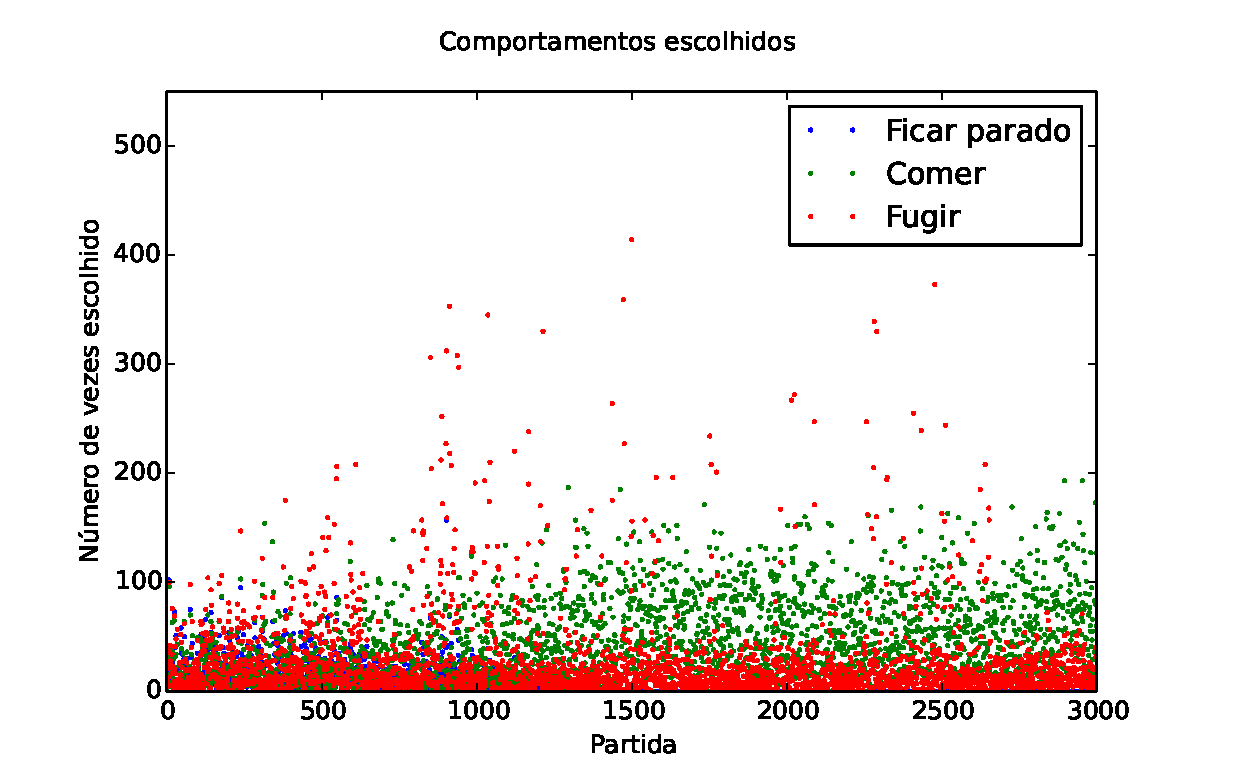
\includegraphics[width=\linewidth]{images/3_behaviors_small_map/chosen_behaviors}
    \caption{Escolha dos comportamentos por partida.}
    \label{img:3ComportamentosMapaPequeno:ComportamentosEscolhidos}
\end{figure}
\end{frame}

%------------------------------------------------

\begin{frame}
\begin{figure}[h]
    \centering
    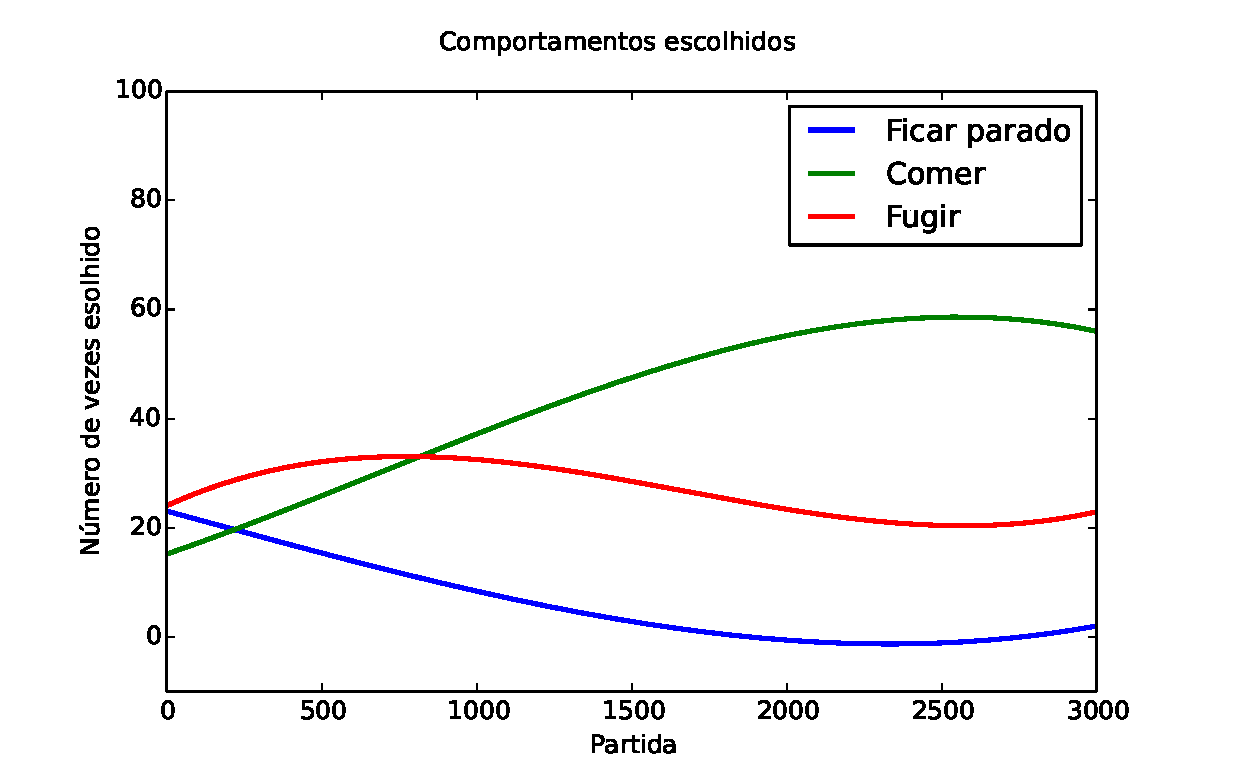
\includegraphics[width=\linewidth]{images/3_behaviors_small_map/chosen_behaviors_pol}
    \caption{Escolha dos comportamentos por partida.}
    \label{img:3ComportamentosMapaPequeno:ComportamentosEscolhidosPolinomio}
\end{figure}
\end{frame}

%------------------------------------------------

\begin{frame}
\begin{figure}[h]
    \centering
    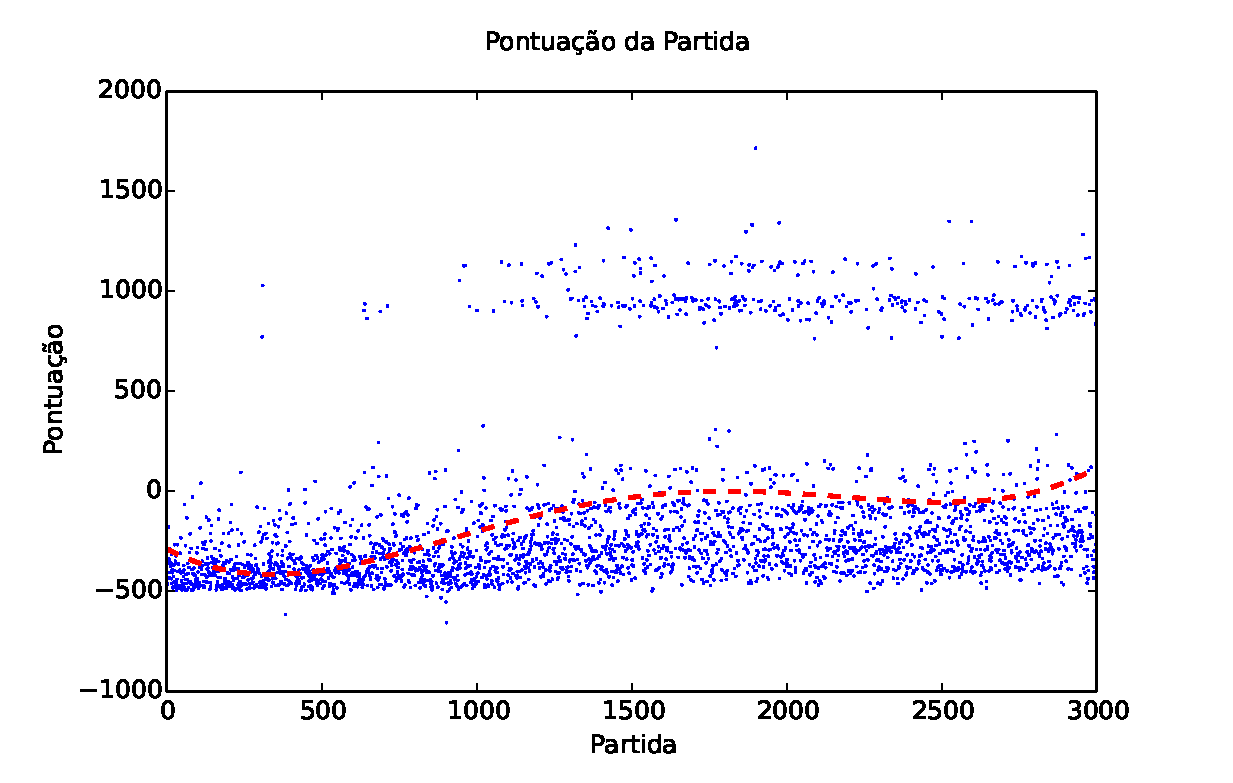
\includegraphics[width=0.7\linewidth]{images/3_behaviors_small_map/match_scores____pol}
    \caption{Pontuação por partida.}
    \label{img:3ComportamentosMapaPequeno:PontuacaoPorPartida}
\end{figure}

Pontuação analisada após a conclusão do treinamento:
$$ \textit{média} \left( \textit{pontuação} \right) = 50.04 $$
\end{frame}

%------------------------------------------------

\subsection{3 Comportamentos no mapa clássico (Teste 2)}

\begin{frame}
Comportamentos:
\begin{itemize}
	\item Ficar Parado;
	\item Comer;
	\item Fugir.
\end{itemize}

\begin{figure}[h]
    \centering
    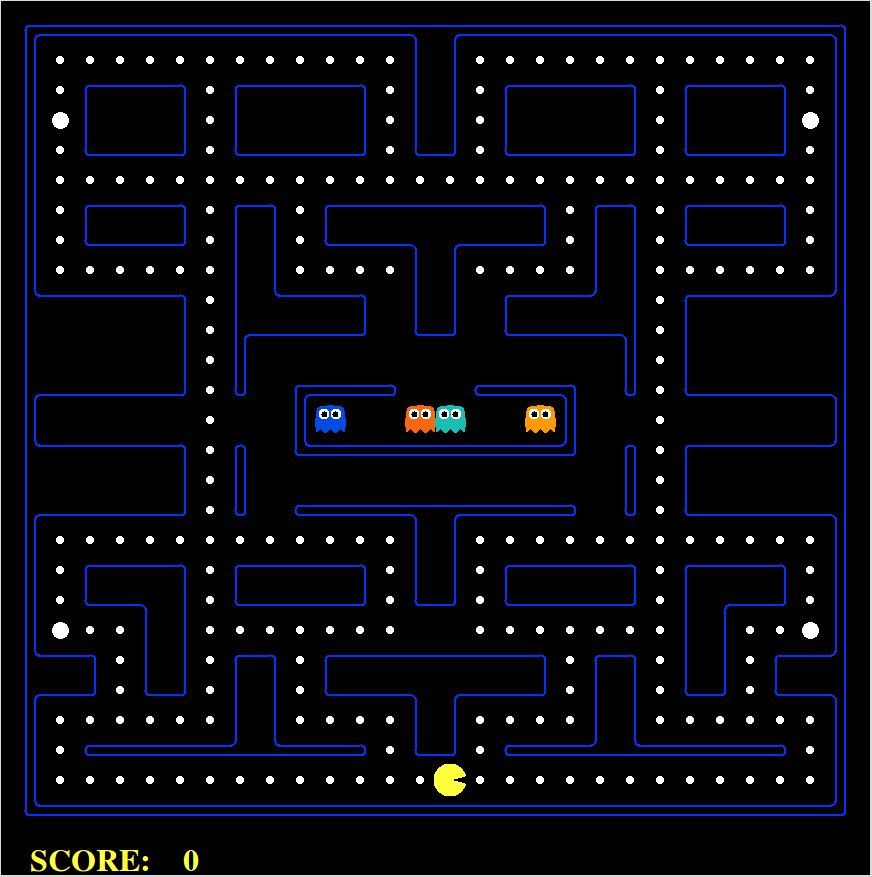
\includegraphics[height=0.6\textheight]{images/pacman_classical_map}
    \caption{Mapa clássico do jogo Pacman.}
    \label{img:PlataformaPacmanMapaClassico}
\end{figure}
\end{frame}

%------------------------------------------------

\begin{frame}
\begin{figure}[H]
    \centering
    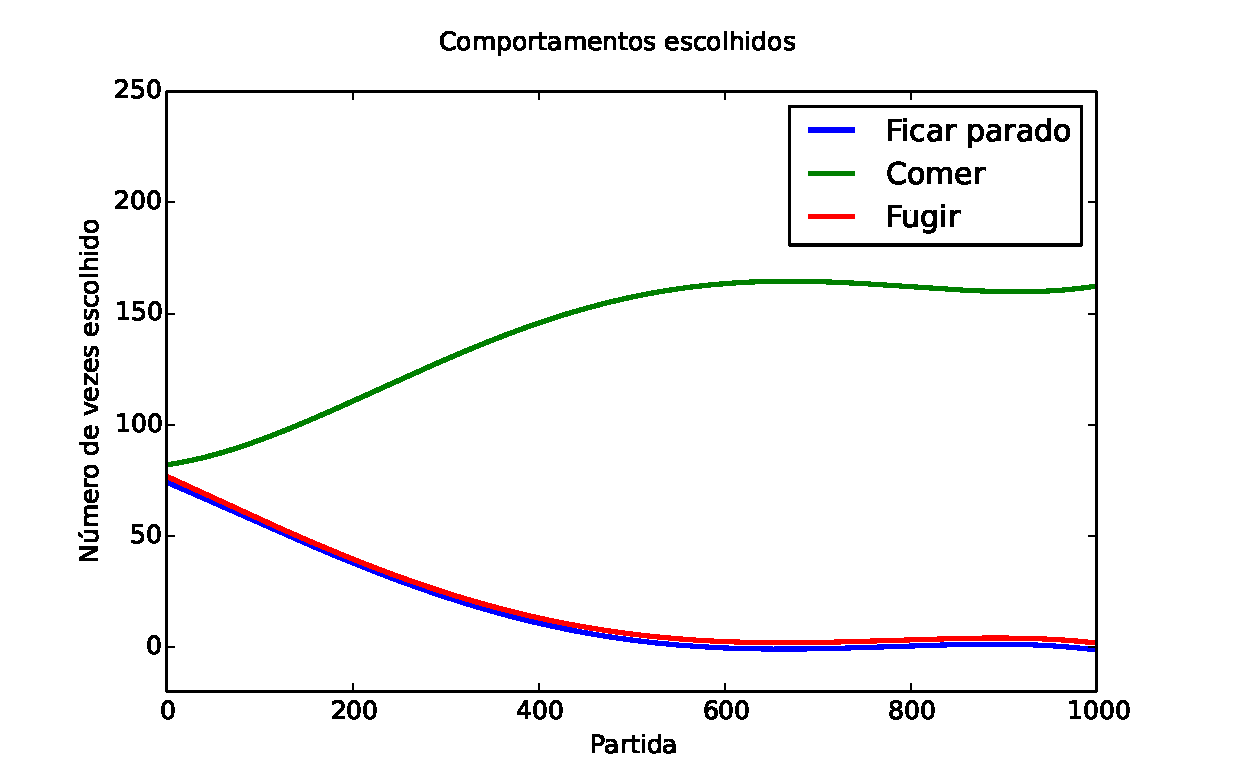
\includegraphics[width=\linewidth]{images/3_behaviors_original_map/chosen_behaviors_pol}
    \caption{Escolha dos comportamentos por partida.}
    \label{img:3ComportamentosMapaOriginal:ComportamentosEscolhidosPolinomio}
\end{figure}
\end{frame}

%------------------------------------------------

\begin{frame}
\begin{figure}[h]
    \centering
    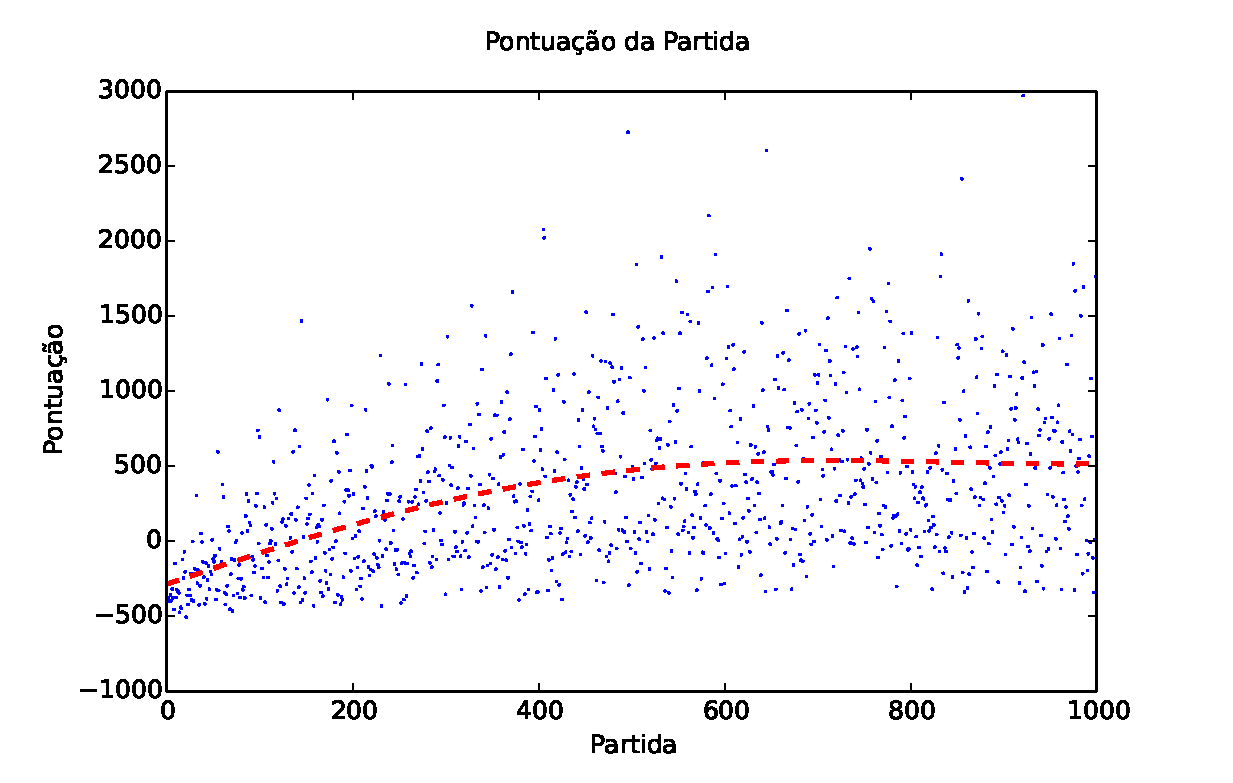
\includegraphics[width=0.7\linewidth]{images/3_behaviors_original_map/match_scores____pol}
    \caption{Pontuação por partida.}
    \label{img:3ComportamentosMapaOriginal:PontuacaoPorPartida}
\end{figure}

Pontuação analisada após a conclusão do treinamento:
$$ \textit{média} \left( \textit{pontuação} \right) = 536.76 $$
\end{frame}

%------------------------------------------------

\subsection{5 Comportamentos no mapa pequeno (Teste 3)}

\begin{frame}
\begin{multicols}{2}
Comportamentos:
\begin{itemize}
	\item Ficar Parado;
	\item Comer;
	\item Fugir;
	\item Comer Cápsula;
	\item Caçar.
\end{itemize}
\vfill
\columnbreak

Características ($ f_i \left( a, B \right) $):
\begin{itemize}
	\item Bias;
	\item Proximidade Comida;
	\item Proximidade Cápsula;
	\item Probabilidade de Fantasma;
	\item Probabilidade de Fantasma Branco.
\end{itemize}

\end{multicols}

\begin{figure}[h]
    \centering
    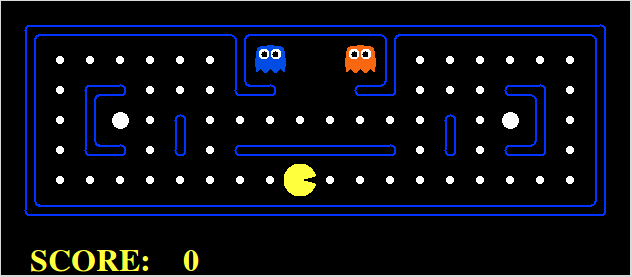
\includegraphics[width=0.6\linewidth]{images/pacman_small_map}
    \caption{Mapa pequeno do jogo Pacman.}
\end{figure}
\end{frame}

%------------------------------------------------

\begin{frame}
\begin{figure}[H]
    \centering
    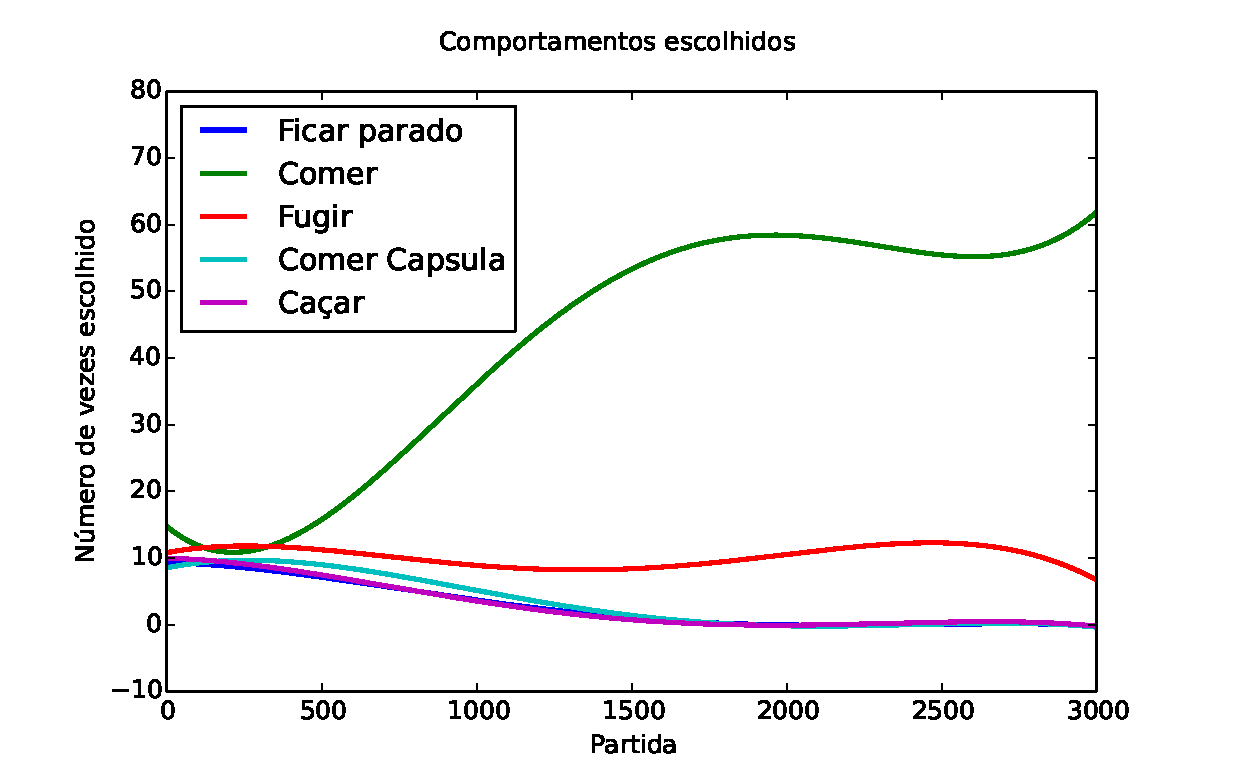
\includegraphics[width=\linewidth]{images/5_behaviors_small_map/chosen_behaviors_pol}
    \caption{Escolha dos comportamentos por partida.}
    \label{img:5ComportamentosMapaPequeno:ComportamentosEscolhidosPolinomio}
\end{figure}
\end{frame}

%------------------------------------------------

\begin{frame}
\begin{figure}[h]
    \centering
    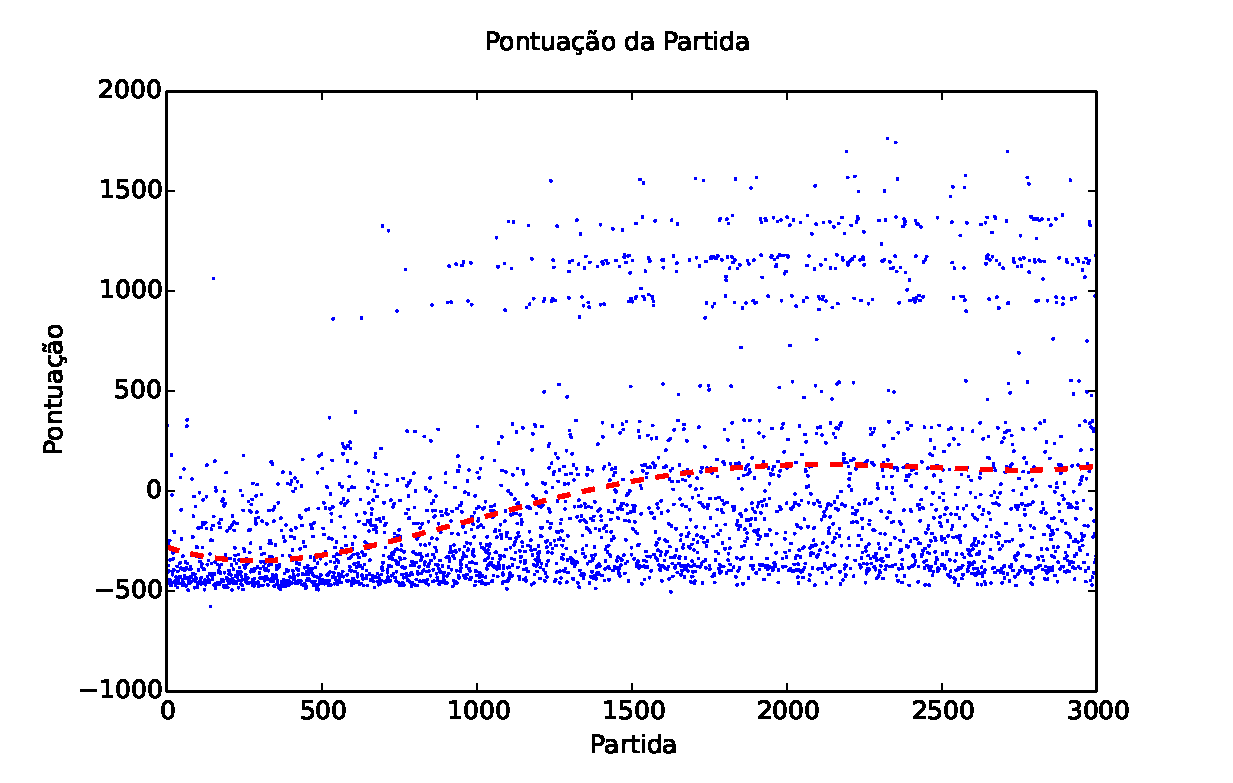
\includegraphics[width=0.7\linewidth]{images/5_behaviors_small_map/match_scores____pol}
    \caption{Pontuação por partida.}
    \label{img:5ComportamentosMapaPequeno:PontuacaoPorPartida}
\end{figure}

Pontuação analisada após a conclusão do treinamento:
$$ \textit{média} \left( \textit{pontuação} \right) = 143.93 $$
\end{frame}

%------------------------------------------------

\subsection{5 Comportamentos no mapa clássico (Teste 4)}

\begin{frame}
Comportamentos:
\begin{itemize}
	\item Ficar Parado;
	\item Comer;
	\item Fugir;
	\item Comer Cápsula;
	\item Caçar.
\end{itemize}

\begin{figure}[h]
    \centering
    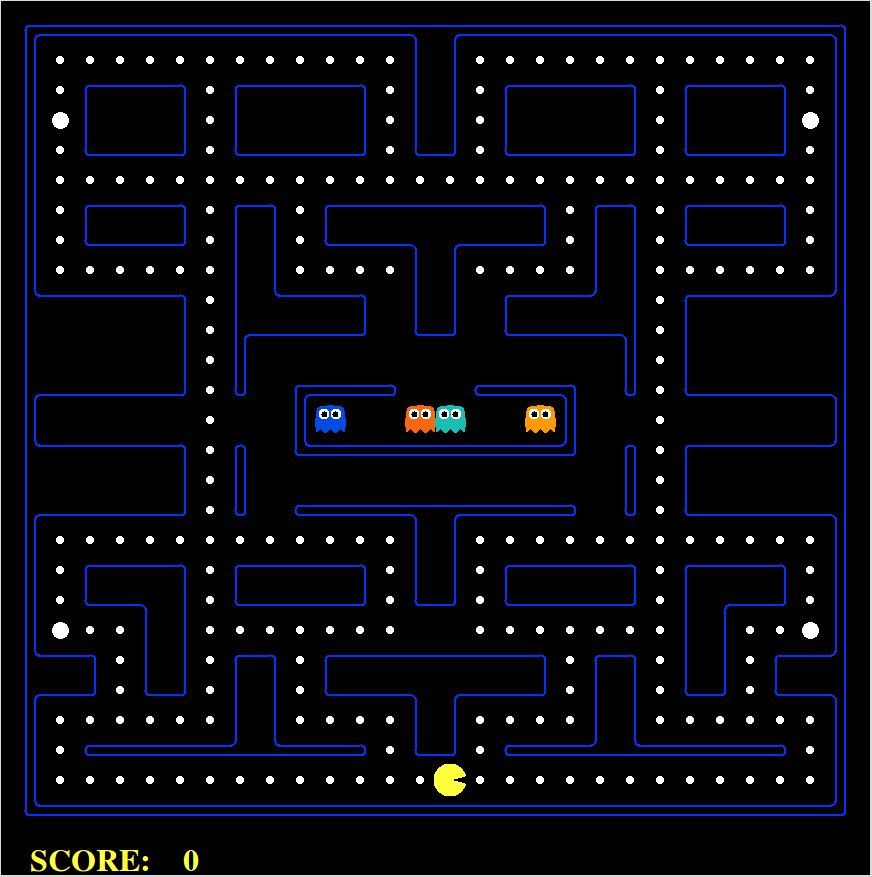
\includegraphics[height=0.5\textheight]{images/pacman_classical_map}
    \caption{Mapa clássico do jogo Pacman.}
\end{figure}
\end{frame}

%------------------------------------------------

\begin{frame}
\begin{figure}[H]
    \centering
    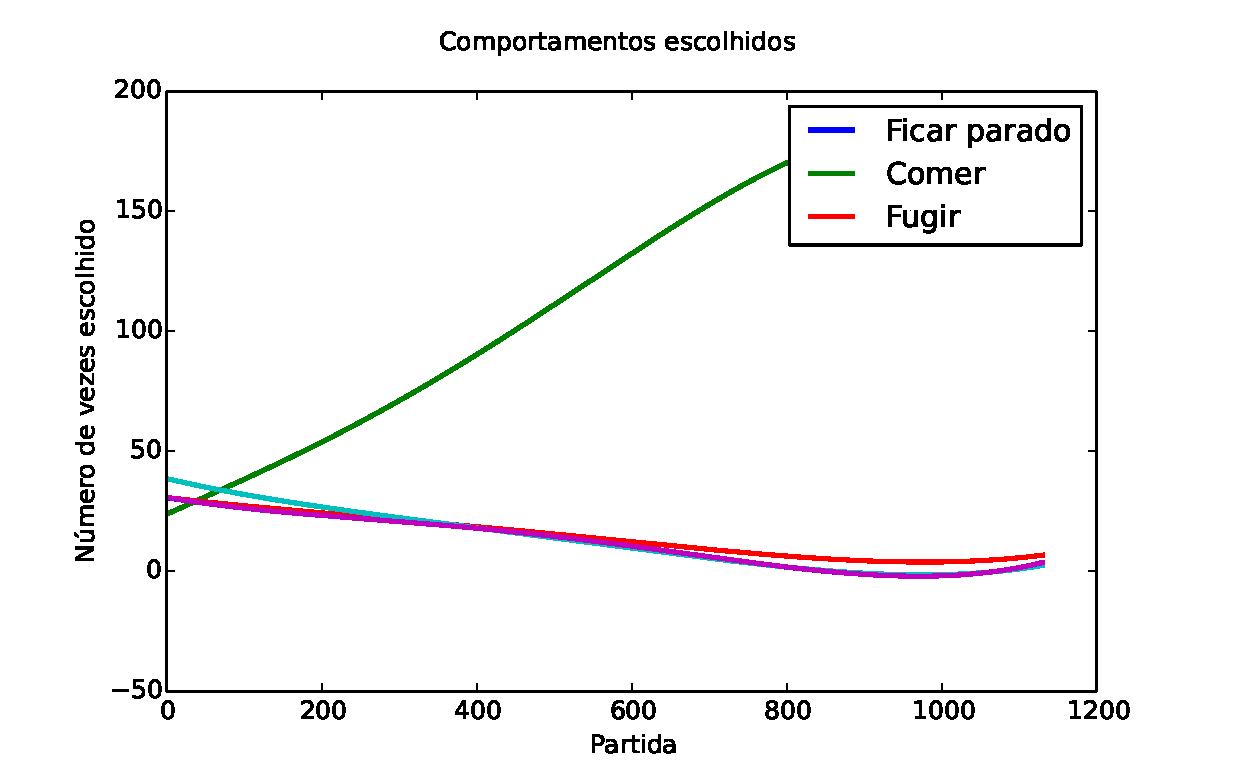
\includegraphics[width=\linewidth]{images/5_behaviors_original_map/chosen_behaviors_pol}
    \caption{Escolha dos comportamentos por partida.}
    \label{img:5ComportamentosMapaOriginal:ComportamentosEscolhidosPolinomio}
\end{figure}
\end{frame}

%------------------------------------------------

\begin{frame}
\begin{figure}[h]
    \centering
    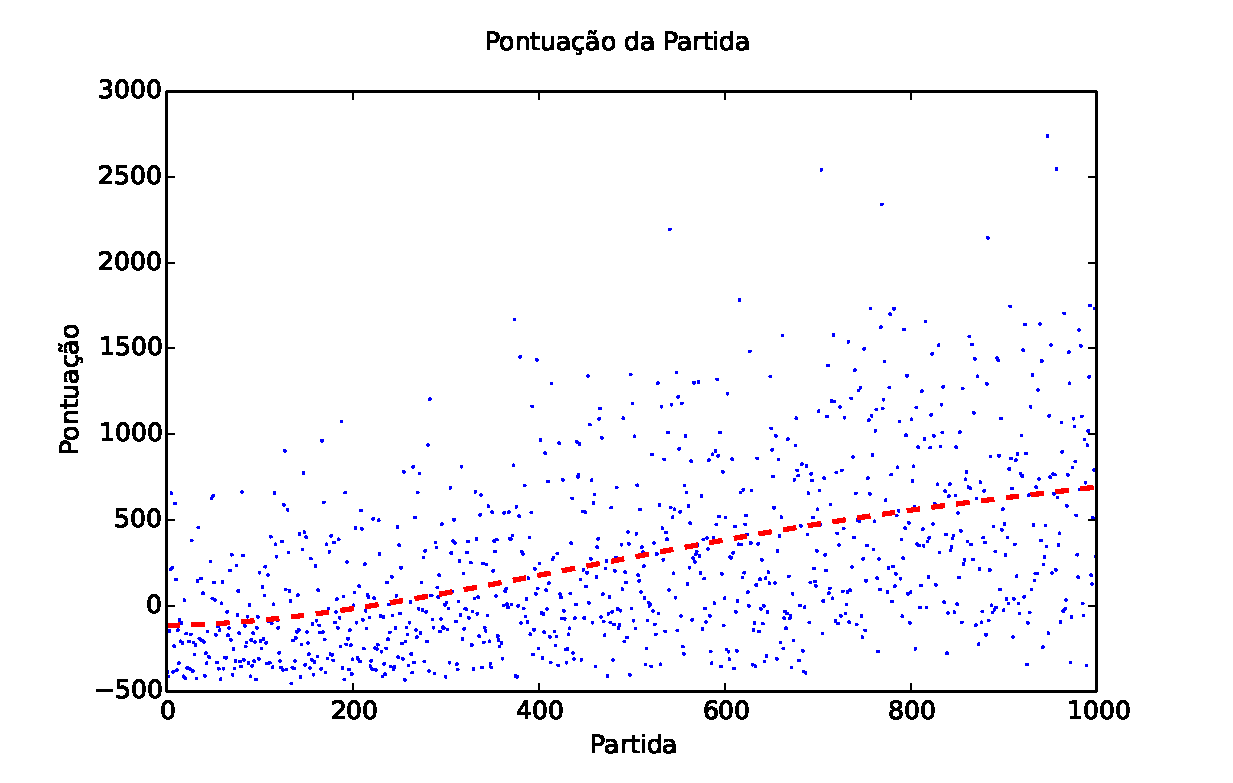
\includegraphics[width=0.7\linewidth]{images/5_behaviors_original_map/match_scores____pol}
    \caption{Pontuação por partida.}
    \label{img:5ComportamentosMapaOriginal:PontuacaoPorPartida}
\end{figure}

Pontuação analisada após a conclusão do treinamento:
$$ \textit{média} \left( \textit{pontuação} \right) = 619.20 $$
\end{frame}

%------------------------------------------------

\begin{frame}
\centerline{\Huge{Conclusões}}
\begin{itemize}
	\item O algoritmo consegue escolher comportamentos de forma lógica;
	\item Foi possível executar tarefas complexas utilizando modelos de seleção de ação simples;
	\item O vetor de características dos pares $ \left( A, B \right) $ deve ser escolhido com cuidado;
	\item O algorítmo possuí certa dificuldade de superar máximos locais.
\end{itemize}
\end{frame}

%------------------------------------------------

\begin{frame}
\bibliographystyle{abnt-num}
\bibliography{presentation}
\end{frame}

\begin{frame}
\Huge{\centerline{Obrigado}}
\end{frame}


%----------------------------------------------------------------------------------------

\end{document} 
